\documentclass[tikz,border=4pt]{standalone}
\usepackage[T1]{fontenc}
\usepackage[utf8]{inputenc}
\usepackage{lmodern}
\usepackage{amsmath,amssymb,mathtools,bm}
\usepackage{graphicx}
\usepackage{booktabs}
\usepackage{array}

\usepackage{tikz}
\usetikzlibrary{arrows.meta,positioning,calc,decorations.pathreplacing,backgrounds,fit,
                shapes.geometric,shapes.misc}
\usepackage{pgfplots}
\pgfplotsset{compat=1.18}
\usepgfplotslibrary{groupplots}

% ---------------------------------------------------------------------
%  PALETTE (light theme of the mid-term presentation)
% ---------------------------------------------------------------------
\definecolor{ink}{RGB}{30,41,59}
\definecolor{muted}{RGB}{100,116,139}
\definecolor{rule}{RGB}{203,213,225}
\definecolor{primary}{RGB}{21,101,146}
\definecolor{teal}{RGB}{34,148,136}
\definecolor{amber}{RGB}{224,122,63}
\definecolor{plum}{RGB}{124,92,168}
\definecolor{panel}{RGB}{238,243,247}
\definecolor{panel2}{RGB}{233,242,240}
\definecolor{cardln}{RGB}{210,222,232}
% methods (the same colours as in every result figure of the report)
\definecolor{cref}{HTML}{2CA02C}
\definecolor{cnone}{HTML}{D62728}
\definecolor{cwhole}{HTML}{FF7F0E}
\definecolor{csub}{HTML}{8C564B}
\definecolor{cocc}{HTML}{1F77B4}
\definecolor{cjoint}{HTML}{9467BD}
% terrain / DEM, unknown scene and data
\definecolor{terrain}{RGB}{120,90,60}
\definecolor{terrainfill}{RGB}{235,228,214}
\definecolor{cunk}{HTML}{C62828}
\definecolor{cdat}{HTML}{1565C0}
% the four channels (one hue, light to dark)
\definecolor{chA}{HTML}{0D47A1}
\definecolor{chB}{HTML}{1E6FCC}
\definecolor{chC}{HTML}{4A94DE}
\definecolor{chD}{HTML}{90C2F0}

\renewcommand{\familydefault}{\sfdefault}
\usepackage{xcolor}
% notation
\newcommand{\dC}{\Delta C_0}
\newcommand{\Nrx}{N_{\mathrm{rx}}}
\newcommand{\PRF}{\mathrm{PRF}}
\newcommand{\PRFop}{\mathrm{PRF}_{\mathrm{op}}}
\newcommand{\bxt}{b_{\mathrm{xt}}}
\newcommand{\bat}{b_{\mathrm{at}}}
\newcommand{\bxti}{b_{\mathrm{xt},i}}
\newcommand{\bati}{b_{\mathrm{at},i}}
\newcommand{\Ba}{B_{\mathrm{a}}}
\newcommand{\jj}{\mathrm{j}}
\newcommand{\ee}{\mathrm{e}}
\newcommand{\Hm}{^{\mathsf H}}
\newcommand{\T}{^{\mathsf T}}
\newcommand{\F}{\mathbf F}
\newcommand{\D}{\mathcal D}
\newcommand{\vg}{\bm g}
\newcommand{\vgh}{\hat{\bm g}}
\newcommand{\gs}{g}
\newcommand{\sv}{{\color{cdat}\bm s}}
\newcommand{\ssv}{{\color{cdat}s}}

\tikzset{
  >={Stealth[length=2.4mm]},
  box/.style   ={rounded corners=3pt,draw=primary,line width=0.9pt,fill=panel,
                 text=ink,align=center,inner sep=4pt,font=\scriptsize},
  tbox/.style  ={rounded corners=3pt,draw=teal,line width=0.9pt,fill=panel2,
                 text=ink,align=center,inner sep=4pt,font=\scriptsize},
  abox/.style  ={rounded corners=3pt,draw=amber,line width=0.9pt,fill=amber!12,
                 text=ink,align=center,inner sep=4pt,font=\scriptsize},
  pbox/.style  ={rounded corners=3pt,draw=plum,line width=0.9pt,fill=plum!10,
                 text=ink,align=center,inner sep=4pt,font=\scriptsize},
  gbox/.style  ={rounded corners=3pt,draw=muted,line width=0.7pt,fill=white,
                 text=ink,align=center,inner sep=4pt,font=\scriptsize},
  dbox/.style  ={rounded corners=3pt,draw=terrain,line width=0.8pt,fill=terrainfill,
                 text=ink,align=center,inner sep=4pt,font=\scriptsize},
  dec/.style   ={diamond,aspect=2.3,draw=amber,line width=0.8pt,fill=amber!14,
                 text=ink,align=center,inner sep=1pt,font=\tiny},
  stepn/.style ={circle,fill=amber,text=white,font=\tiny\bfseries\sffamily,inner sep=0.6pt,minimum size=3.9mm},
  arr/.style   ={-{Stealth[length=2.2mm]},line width=0.9pt,draw=muted},
  bx/.style    ={rounded corners=2pt,line width=0.8pt,align=center,inner sep=2.5pt,text width=#1},
  bx/.default=3.2cm,
  lane/.style  ={rounded corners=5pt,line width=0.7pt},
  ln/.style    ={anchor=north,align=center,font=\footnotesize},
  tarr/.style  ={-{Stealth[length=2.2mm]},line width=1.0pt,draw=teal},
  aarr/.style  ={-{Stealth[length=2.2mm]},line width=1.0pt,draw=amber},
  parr/.style  ={-{Stealth[length=2.2mm]},line width=1.0pt,draw=plum},
  cota/.style  ={<->,line width=0.5pt,draw=muted},
  brc/.style   ={decorate,decoration={brace,amplitude=4pt},draw=muted,line width=0.6pt},
  nota/.style  ={font=\scriptsize,text=muted,align=center},
  % operators of the joint model, coloured by the domain in which they act
  op/.style    ={draw=muted,fill=white,rounded corners=2pt,align=center,inner sep=2.5pt,
                 minimum height=8mm,minimum width=10mm,font=\small,line width=0.6pt},
  opx/.style   ={op,draw=teal,fill=panel2},      % position (focused line)
  opf/.style   ={op,draw=primary,fill=panel},    % Doppler frequency
  opt/.style   ={op,draw=amber,fill=amber!10},   % time (raw channel line)
  sat/.style   ={circle,draw=ink,fill=white,line width=0.8pt,inner sep=2pt},
}


% ---------------------------------------------------------------------------------------------- helpers
\tikzset{
  invisible/.style={opacity=0,text opacity=0},
  visible on/.style={alt={#1{}{invisible}}},
  alt/.code args={<#1>#2#3}{\alt<#1>{\pgfkeysalso{#2}}{\pgfkeysalso{#3}}},
  gvisible on/.style={alt={#1{}{transparency group,opacity=0}}},
  nohyph/.style={execute at begin node={\hyphenpenalty=10000\exhyphenpenalty=10000}},
  pillst/.style={rounded corners=4.5pt,inner xsep=4.5pt,inner ysep=1.6pt,font=\scriptsize\sffamily\bfseries},
  lbl/.style={font=\scriptsize,text=ink},
  mlbl/.style={font=\scriptsize,text=muted},
}
\definecolor{sl0}{HTML}{E2E8F0}\definecolor{sl1}{HTML}{CBD5E1}\definecolor{sl2}{HTML}{94A3B8}\definecolor{sl3}{HTML}{64748B}
\newcommand{\pilltw}{\tikz[baseline=-0.62ex]\node[pillst,fill=primary!14,text=primary]{this work};}
\newcommand{\cfg}[1]{\framesubtitle{#1}}
\newcommand{\cfgp}[2]{\framesubtitle{#2\hfill#1}}
\newcommand{\dt}{\enspace$\cdot$\enspace}
\newcommand{\lyr}[2]{\node<#1>[anchor=north west,inner sep=0pt] at (0,0) {\includegraphics{figures/v20/#2}};}
% phase dial: centre (#1,#2), radius #3; arrow at #4 degrees clockwise from 12 o'clock, colour #5
\newcommand{\dialbase}[3]{\draw[rule,line width=0.6pt,fill=white] (#1,#2) circle (#3);
  \draw[muted,line width=0.6pt] (#1,#2+#3) -- (#1,#2+0.78*#3);}
\newcommand{\dialarc}[5]{\draw[#5,line width=0.8pt] ($(#1,#2)+(90:{0.58*#3})$) arc[start angle=90,end angle={90-(#4)},radius={0.58*#3}];}
\newcommand{\dialarrow}[5]{\draw[-{Stealth[length=1.9mm,width=1.8mm]},line width=1.2pt,#5] (#1,#2) -- ++({90-(#4)}:{0.84*#3});}
% slide 9: the scatterer on the iso-range arc of the Tx (angle #1 seen from the Tx), #2 > 0: label it
\newcommand{\scat}[2]{%
  \coordinate (P) at ($(Tx)+(#1:\rr)$);
  \draw[primary,line width=0.9pt] (Tx) -- (P);
  \draw[chB,line width=0.9pt] (Rx) -- (P);
  \ifnum#2>1 \draw[cota] (P |- 0,\zg) -- node[right=-1pt]{$h$} (P); \fi
  \ifnum#2>0 \node[anchor=west] at ($(P)+(0.25,0.1)$) {scatterer}; \fi
  \fill[ink] (P) circle (2.3pt);}


% ---------------------------------------------------------------------------------------------- v28 helpers
% styles of the joint algorithm (overview, stage slides and closing)
\tikzset{
  pa/.style={rounded corners=2pt,line width=0.8pt,draw=ink!55,fill=white,align=center,text width=2.35cm,
             inner sep=2.2pt,minimum height=1.55cm,nohyph},
  lo/.style={rounded corners=2pt,line width=0.8pt,draw=primary,fill=panel,align=center,text width=2.1cm,
             inner sep=2.2pt,minimum height=1.0cm,nohyph},
  fi/.style={rounded corners=2pt,line width=0.8pt,draw=plum,fill=plum!10,align=center,text width=3.0cm,inner sep=2.2pt,
             nohyph},
  io/.style={rounded corners=2pt,line width=0.8pt,draw=muted,fill=muted!8,align=center,inner sep=2.2pt,nohyph},
  bd/.style={circle,fill=amber,text=white,font=\scriptsize\bfseries\sffamily,inner sep=0pt,minimum size=5.0mm},
  parr2/.style={-{Stealth[length=2.2mm]},line width=1.0pt,draw=primary},
  lanelab/.style={anchor=west,align=left,text width=2.0cm,font=\footnotesize\bfseries,nohyph},
}
\newcommand{\jointstyles}{}
% "you are here": a thumbnail of the overview (three lanes) in the top-right corner, below the title rule;
% #1 = comma list of the lit cells: P1,P2,P3,P4,L (the loop),F1,F2
\makeatletter
\newcommand{\yhcell}[5]{% name, x, y, width, label
  \edef\yh@do{\noexpand\in@{,#1,}{,\yhlist,}}\yh@do
  \ifin@\node[draw=amber,fill=amber,text=white,minimum width=#4cm,minimum height=0.27cm,inner sep=0pt,rounded corners=1pt]
     at (#2,#3) {#5};
  \else\node[draw=rule,fill=white,text=muted,minimum width=#4cm,minimum height=0.27cm,inner sep=0pt,rounded corners=1pt]
     at (#2,#3) {#5};\fi}
\makeatother
\newcommand{\youarehere}[1]{%
  \def\yhlist{#1}%
  \begin{tikzpicture}[remember picture,overlay]
    \begin{scope}[shift={([xshift=-3.25cm,yshift=-2.75cm]current page.north east)},x=1cm,y=1cm,
                  font=\fontsize{5}{5}\selectfont\sffamily\bfseries]
      \fill[muted!5,rounded corners=1.5pt] (0,0.9) rectangle (2.65,1.3); \draw[ink!40,rounded corners=1.5pt,line width=0.4pt] (0,0.9) rectangle (2.65,1.3);
      \fill[panel!60,rounded corners=1.5pt] (0,0.45) rectangle (2.65,0.85); \draw[primary,rounded corners=1.5pt,line width=0.4pt] (0,0.45) rectangle (2.65,0.85);
      \fill[plum!6,rounded corners=1.5pt] (0,0) rectangle (2.65,0.4); \draw[plum,rounded corners=1.5pt,line width=0.4pt] (0,0) rectangle (2.65,0.4);
      \yhcell{P1}{0.42}{1.1}{0.52}{P1}\yhcell{P2}{1.02}{1.1}{0.52}{P2}\yhcell{P3}{1.62}{1.1}{0.52}{P3}\yhcell{P4}{2.22}{1.1}{0.52}{P4}
      \yhcell{L}{1.32}{0.65}{2.32}{S1--S3 loop}
      \yhcell{F1}{0.72}{0.2}{1.12}{F1}\yhcell{F2}{1.92}{0.2}{1.12}{F2}
    \end{scope}
  \end{tikzpicture}}

% ---- v28: the five factors of the model s_i = D H_i K Psi_i g, one colour each, the same on every joint slide
%      (never red / green / purple: those mean standard / reference / joint reconstruction)
\colorlet{fD}{amber!88!black}\colorlet{fH}{primary}\definecolor{fK}{HTML}{5B6B85}\colorlet{fP}{terrain}\colorlet{fG}{ink}
\newcommand{\fD}{{\color{fD}D}}\newcommand{\fH}{{\color{fH}H_i}}\newcommand{\fK}{{\color{fK}K}}
\newcommand{\fKi}{{\color{fK}K_i}}\newcommand{\fP}{{\color{fP}\Psi_i}}
\newcommand{\modelA}{\mathbf A_i=\fD\cdot\fKi\cdot\fP}
% ---- v28: the simulation parameters, the same grey block under the title of every result slide; #1 = what is
%      specific to the slide
\newcommand{\simline}{$N_{\mathrm{rx}}=4$ (Rx0 $=$ Tx)\dt 500\,Hz each (2000\,Hz together)\dt
  $\bxt=300,\ 119.8,\ 100.5$\,m\dt $\lambda=0.25$\,m\dt $v=7689$\,m/s\dt $r_0=766$\,km}
\newcommand{\simcfg}[1]{\framesubtitle{\simline\\ look angle $20^\circ$\dt $\Ba=1235$\,Hz\dt #1}}

% standalone: every build step shown
\tikzset{visible on/.style={},gvisible on/.style={}}
\providecommand{\vstrip}[5]{\foreach \c in {1,...,#3}
  \draw[#5,line width=0.5pt] ({#1+(\c-1)*#4},{#2-0.17}) rectangle ({#1+\c*#4},{#2+0.17});}

% What channel i records: s_i = D H_i K Psi_i g, read right to left
\begin{document}
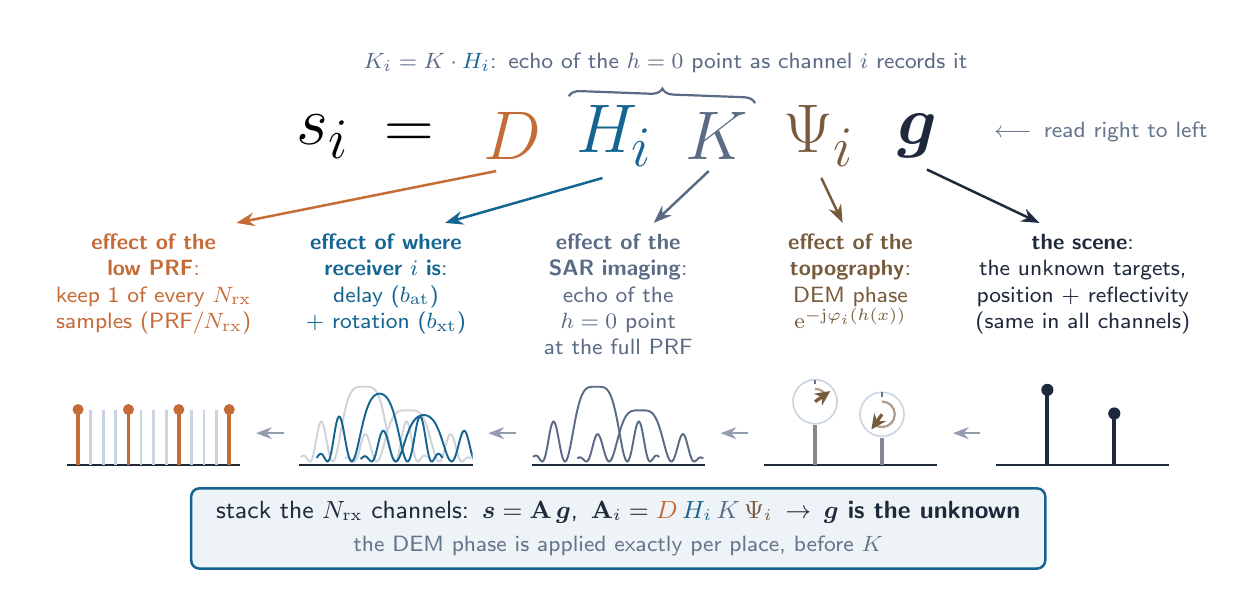
\begin{tikzpicture}[font=\footnotesize]
    \path (0,-1.0) rectangle (15.0,6.0);
    \def\ye{4.62}\def\yc{3.42}\def\yp{0.85}
    \def\xD{1.6}\def\xH{4.55}\def\xK{7.5}\def\xP{10.45}\def\xG{13.4}
    \tikzset{meq/.style={font=\fontsize{30}{30}\selectfont,inner sep=1pt},
             mcap/.style={anchor=north,align=center,text width=2.8cm,inner sep=1pt,nohyph},
             mfa/.style={-{Stealth[length=2.3mm]},line width=0.9pt},
             mflow/.style={-{Stealth[length=2.0mm]},line width=0.9pt,draw=muted!70}}
    % ---- the equation: every factor grey until its step
    \node[meq] at (3.75,\ye) {$s_i$}; \node[meq] at (4.85,\ye) {$=$};
    \node[meq,text=fD] (eD) at (6.15,\ye) {$D$};
    \node[meq,text=fH] (eH) at (7.45,\ye) {$H_i$};
    \node[meq,text=fK] (eK) at (8.75,\ye) {$K$};
    \node[meq,text=fP] (eP) at (10.05,\ye) {$\Psi_i$};
    \node[meq,text=fG] (eG) at (11.3,\ye) {$\vg$};
    \node[anchor=west,text=muted,font=\footnotesize] at (12.15,\ye+0.05) {$\longleftarrow$\enspace read right to left};
    % ---- step 1: g, the scene
    \node[mcap,text=fG] (cG) at (\xG,\yc) {\textbf{the scene}:\\ the unknown targets,\\ position + reflectivity\\ (same in all channels)};
    \draw[mfa,fG] ($(eG.south)+(0.12,-0.1)$) -- ($(cG.north)+(-0.55,0.1)$);
    \begin{scope}[shift={(\xG,\yp)}]
      \draw[ink,line width=0.6pt] (-1.1,-0.4) -- (1.1,-0.4);
      \foreach \x/\a in {-0.45/0.95,0.4/0.65} {\draw[fG,line width=1.4pt] (\x,-0.4) -- (\x,-0.4+\a); \fill[fG] (\x,-0.4+\a) circle (2.2pt);}
    \end{scope}
    % ---- step 2: Psi_i, the DEM phase of each place
    \begin{scope}[visible on=<2->]
      \node[mcap,text=fP] (cP) at (\xP,\yc) {\textbf{effect of the}\\ \textbf{topography}:\\ DEM phase\\ $\ee^{-\jj\varphi_i(h(x))}$};
      \draw[mfa,fP] ($(eP.south)+(0.03,-0.1)$) -- ($(cP.north)+(-0.1,0.1)$);
      \draw[mflow] (\xG-1.3,\yp) -- (\xP+1.3,\yp);
      \begin{scope}[shift={(\xP,\yp)}]
        \draw[ink,line width=0.6pt] (-1.1,-0.4) -- (1.1,-0.4);
        \foreach \x/\a/\ang in {-0.45/0.5/55,0.4/0.34/215}{
          \draw[fG!55,line width=1.4pt] (\x,-0.4) -- (\x,-0.4+\a);
          \dialbase{\x}{-0.4+\a+0.3}{0.28} \dialarc{\x}{-0.4+\a+0.3}{0.28}{\ang}{fP!60} \dialarrow{\x}{-0.4+\a+0.3}{0.28}{\ang}{fP}}
      \end{scope}
    \end{scope}
    % ---- step 3: K (the echo of the h = 0 point) and H_i (channel i); together K_i
    \begin{scope}[visible on=<3->]
      \node[mcap,text=fK] (cK) at (\xK,\yc) {\textbf{effect of the}\\ \textbf{SAR imaging}:\\ echo of the \mbox{$h=0$} point\\ at the full PRF};
      \draw[mfa,fK] ($(eK.south)+(-0.1,-0.1)$) -- ($(cK.north)+(0.45,0.1)$);
      \node[mcap,text=fH] (cH) at (\xH,\yc) {\textbf{effect of where}\\ \textbf{receiver $i$ is}:\\ delay ($\bat$)\\ + rotation ($\bxt$)};
      \draw[mfa,fH] ($(eH.south)+(-0.15,-0.1)$) -- ($(cH.north)+(0.75,0.1)$);
      \draw[mflow] (\xP-1.3,\yp) -- (\xK+1.3,\yp); \draw[mflow] (\xK-1.3,\yp) -- (\xH+1.3,\yp);
      \begin{scope}[shift={(\xK,\yp)}]
        \draw[ink,line width=0.6pt] (-1.1,-0.4) -- (1.1,-0.4);
        \clip (-1.1,-0.45) rectangle (1.1,0.75);
        \foreach \c/\a in {-0.28/0.95,0.28/0.65}
          \draw[fK,line width=0.7pt] plot[domain=-0.8:0.8,samples=120,smooth] ({\c+\x},{-0.36+0.5*\a*(1+cos(deg(2*pi*3.2*\x*\x)))*exp(-0.5*(\x/0.52)^4)});
      \end{scope}
      \begin{scope}[shift={(\xH,\yp)}]
        \draw[ink,line width=0.6pt] (-1.1,-0.4) -- (1.1,-0.4);
        \clip (-1.1,-0.45) rectangle (1.1,0.75);
        \foreach \c/\a in {-0.28/0.95,0.28/0.65}
          \draw[fK!30,line width=0.7pt] plot[domain=-0.8:0.8,samples=120,smooth] ({\c+\x},{-0.36+0.5*\a*(1+cos(deg(2*pi*3.2*\x*\x)))*exp(-0.5*(\x/0.52)^4)});
        \foreach \c/\a in {-0.28/0.95,0.28/0.65}
          \draw[fH,line width=0.7pt] plot[domain=-0.8:0.8,samples=120,smooth] ({\c+0.2+\x},{-0.36+0.5*\a*(1+cos(deg(2*pi*3.2*\x*\x+120)))*exp(-0.5*(\x/0.52)^4)});
      \end{scope}
      \draw[brc,draw=fK,line width=0.8pt] ($(eH.north west)+(-0.05,0.08)$) -- ($(eK.north east)+(0.05,0.08)$);
      \node[anchor=south,font=\footnotesize,text=fK] at ($(eH.north)!0.5!(eK.north)+(0,0.3)$)
        {$K_i=K\cdot{\color{fH}H_i}$:\enspace echo of the \mbox{$h=0$} point as channel $i$ records it};
    \end{scope}
    % ---- step 4: D (one sample in N_rx), then the stack of the channels
    \begin{scope}[visible on=<4->]
      \node[mcap,text=fD] (cD) at (\xD,\yc) {\textbf{effect of the}\\ \textbf{low PRF}:\\ keep 1 of every $N_{\mathrm{rx}}$\\ samples (PRF$/N_{\mathrm{rx}}$)};
      \draw[mfa,fD] ($(eD.south)+(-0.2,-0.1)$) -- ($(cD.north)+(1.05,0.1)$);
      \draw[mflow] (\xH-1.3,\yp) -- (\xD+1.3,\yp);
      \begin{scope}[shift={(\xD,\yp)}]
        \draw[ink,line width=0.6pt] (-1.1,-0.4) -- (1.1,-0.4);
        \foreach \k in {0,...,12}{
          \pgfmathsetmacro{\xx}{-0.96+0.16*\k}
          \pgfmathtruncatemacro{\kq}{mod(\k,4)==0 ? 1 : 0}
          \ifnum\kq=1 \draw[fD,line width=1.3pt] (\xx,-0.4) -- (\xx,0.3); \fill[fD] (\xx,0.3) circle (2.0pt);
          \else \draw[rule,line width=1.0pt] (\xx,-0.4) -- (\xx,0.3); \fi}
      \end{scope}
      \node[box,font=\small,inner xsep=9pt,inner ysep=4.5pt,align=center] at (7.5,-0.36)
        {stack the $N_{\mathrm{rx}}$ channels:\enspace $\bm s=\mathbf A\,\vg$,\enspace $\mathbf A_i=\fD\,\fH\,\fK\,\fP$\enspace $\to$\enspace
         \textbf{$\vg$ is the unknown}\\[0.3ex]
         {\footnotesize\color{muted}the DEM phase is applied exactly per place, before $K$}};
    \end{scope}
  \end{tikzpicture}
\end{document}
